\documentclass{article}
\usepackage{amsmath}
\usepackage{graphicx}

\begin{document}
\section{Primary Flux Environment}



%%%%%%%%%%%%%%%%%%%%%%%%%%%%%%%%%%%%%%%%%%%%%%%%%%%%%%%%%%%%%%%%%%%%%%
\subsection{Space-Time Dependence of Environment}

The primary environment that is responsible for creating ejecta by impacting the lunar surface varies in both location on the Moon as well as in time. For a time-averaged background environment, the sporadic meteoroid complex (Section \ref{ssec:Sporadic Meteoroid Complex}) and near-Earth object (Section \ref{ssec:Near-Earth Objects}) populations are used as input to the ejecta model over a 19-year time span. Short-term environments may also be generated that have the option to include the meteor showers (Section \ref{ssec:Meteoroid Showers}, forward work). Time-varying environments can also be generated by providing consecutive ephemeris definitions in time. If a single time frame is used, it is thought of as the average environment over that time frame.

The location and time span of the primary environment is defined by an ephemeris, or trajectory file, discussed in Section \ref{sssec:Ephemeris Definition}.

%%%%%%%%%%%%%%%%%%%%%%%%%%%%%%%%%%%%%%%%%%%%%%%%%%%%%%%%%%%%%%%%%%%%%%
\subsubsection{Ephemeris Definition}\label{sssec:Ephemeris Definition}

The ephemeris definitions of locations on the Moon are generated by using the service provided by JPL Horizons at \url{ssd.jpl.nasa.gov/horizons/}. One way to query their system is to send an email that defines the particular inputs desired, e.g., see Listing~\ref{lst:JPL horizons send email}, which makes it easier to streamline generating many ephemeris files quickly.

\lstinputlisting[language={}, label={lst:JPL horizons send email}, basicstyle=\small, caption={An example email that is sent to JPL Horizons to compute an ephemeris file that is centered on the Moon at a location of $90^\circ$ longitude, $-65^\circ$ latitude, and $0.6$ km above the surface for 11 years.}]{example_email_jpl_horizons.txt}

In order to convert the ephemeris file received from JPL Horizons to a file type that the Meteoroid Engineering Model (MEM) program can read, a Python script is used as shown in Listing \ref{lst:python ephemeris converter}.

\lstinputlisting[language={python}, label={lst:python ephemeris converter}, basicstyle=\footnotesize, caption={Python script to convert JPL Horizons ephemeris file type to be read into the Meteoroid Engineering Model.}]{../LunarSurfaceEphemerisData_Meridian/ephemeris_parser.py}

Several ephemeris files can be used to define local primary environments on the Moon by specifying different latitude-longitude coordinates. As an example, $5$-degree increments can be used in latitude going from the north pole\footnote{The poles must not be exactly $\pm 90^\circ$, but offset slightly to avoid errors in the JPL Horizons system.} ($+90^\circ$) to the south pole ($-90^\circ$) and $90$-degrees increments can be used in longitude to define the meridian ($0^\circ$), eastern limb ($+90^\circ$), far side ($+180^\circ$), and the western limb ($+270^\circ$) locations.

%%%%%%%%%%%%%%%%%%%%%%%%%%%%%%%%%%%%%%%%%%%%%%%%%%%%%%%%%%%%%%%%%%%%%%
%\subsubsection{Selenographic Extent}


%%%%%%%%%%%%%%%%%%%%%%%%%%%%%%%%%%%%%%%%%%%%%%%%%%%%%%%%%%%%%%%%%%%%%%
\subsection{Sporadic Meteoroid Complex}\label{ssec:Sporadic Meteoroid Complex}


The primary flux of sporadic meteoroids onto the surface of the Moon changes depending on the selenographic location on the Moon. Because of this effect, ephemeris data\footnote{Horizons Ephemeris System $<$horizons@ssd.jpl.nasa.gov$>$.} was generated for different latitudes and longitudes on the Moon in 5-degree increments from pole to pole, and in 90-degree increments in longitude. A time frame of 19 years was chosen, or a Metonic cycle, which takes into account many different Sun-Earth-Moon geometries. The Meteoroid Engineering Model (MEM) \citep{moorhead2019nasa} is used to generate the sporadic meteoroids, i.e., the background flux.

\begin{figure}[!htb]
	\begin{subfigure}{.485\textwidth}
		\centering
		% include first image
		\includegraphics[width=.85\linewidth]{../LoDensity018_lat0.png}  
		\caption{Low density population impacting at the equator.}
		\label{fig:sub-LoDensity018_lat0}
	\end{subfigure}
	\begin{subfigure}{.485\textwidth}
		\centering
		% include second image
		\includegraphics[width=.85\linewidth]{../LoDensity036_lat90.png}  
		\caption{Low density population impacting at the north pole.}
		\label{fig:sub-LoDensity036_lat90}
	\end{subfigure}
	\newline
	\begin{subfigure}{.485\textwidth}
		\centering
		% include third image
		\includegraphics[width=.85\linewidth]{../HiDensity018_lat0.png}  
		\caption{High density population impacting at the equator.}
		\label{fig:sub-HiDensity018_lat0}
	\end{subfigure}
	\begin{subfigure}{.485\textwidth}
		\centering
		% include fourth image
		\includegraphics[width=.85\linewidth]{../HiDensity036_lat90.png}  
		\caption{High density population impacting at the north pole.}
		\label{fig:sub-HiDensity036_lat90}
	\end{subfigure}
	\caption{Fluxes at the meridional plane (as a function of impact speed and angle from the horizon) of the low density population (a) and (b), and the high density population (c) and (d) impacting the Moon at the equator (a) and (c), and the north/south pole (b) and (d).}
	\label{fig:latitudinal_dependence}
\end{figure}

As an example, in Figure \ref{fig:latitudinal_dependence}, the speed-angle flux distribution is shown at the equator and at the poles for the low and high density MEM populations. Note that the fluxes in the northern and southern hemispheres are symmetric about the equator. It can be seen from Figure \ref{fig:latitudinal_dependence} that the impact angles and speeds are highly dependent on the impact latitude on the Moon and hence warrant a more sophisticated approach to computing the secondary fluxes. It cannot be assumed that most impacts are at 45~degrees or are not highly oblique.% How this latitude dependence affects the secondary flux is not entirely clear, except for the fact that we hypothesize that the secondary fluxes will be themselves dependent on latitude.
%\clearpage

Other time frames may be simulated, such a week, a month, or a year, and can also vary as a function of time. In the current model output, a 19-year averaged flux is used.


%%%%%%%%%%%%%%%%%%%%%%%%%%%%%%%%%%%%%%%%%%%%%%%%%%%%%%%%%%%%%%%%%%%%%%
\subsubsection{Angular Distribution}

The angular distribution of the primary fluxes can be viewed in a Mollweide and all-sky (polar) projection for both the low- and high-density components of the sporadic meteoroids. Three specific latitudinal regions are depicted in Figures \ref{fig:MEM angular dist at poles}, \ref{fig:MEM angular dist at 45 deg}, and \ref{fig:MEM angular dist at equator} for the south pole, $-45^\circ$ latitude, and the equator, respectively, at the central meridian ($0^\circ$ longitude).

The fluxes from the low- and high-density components seem to originate from opposing locations in the sky \citep[e.g., see Figure 2.2 of][]{moorhead2019nasa}. The shift is due to the high-density population meteoroids coming from mainly the ecliptic plane (helion and anti-helion sources) while the low-density population tends to come from higher inclinations (toroidal and apex sources).

The figures that follow show a departure from a purely isotropic flux source and the effect on the impact angle on the planetary surface. As shown in \cite{pierazzo2000understanding}, the probability of hitting a planetary body, regardless of the target's gravitational field, is given by
\begin{equation}
dP = 2\sin\alpha\cos\alpha d\alpha,
\end{equation}
where $\alpha$ is the angle from zenith. This equation shows that the most probable impact angle is at $45^\circ$, which is not supported by the sporadic meteoroid fluxes, implying a non-isotropic origin -- known to be the helion/anti-helion, toroidal, and apex sources.



\begin{figure}[!htb]
	\begin{subfigure}{.485\textwidth}
		\centering
		% include first image
		\includegraphics[width=.85\linewidth]{../mollweide_LatRunDataLoDensity000_lat-90.png}  
		\caption{Mollweide view of the low density population impacting at the south pole.}
		\label{fig:mollweide_LatRunDataLiDensity000_lat-90}
	\end{subfigure}
	\begin{subfigure}{.485\textwidth}
		\centering
		% include second image
		\includegraphics[width=.85\linewidth]{../polar_LatRunDataLoDensity000_lat-90.png}  
		\caption{All-sky view of the low density population impacting at the south pole.}
		\label{fig:polar_LatRunDataLoDensity000_lat-90}
	\end{subfigure}
	\newline
	\begin{subfigure}{.485\textwidth}
		\centering
		% include third image
		\includegraphics[width=.85\linewidth]{../mollweide_LatRunDataHiDensity000_lat-90.png}  
		\caption{Mollweide view of the high density population impacting at the south pole.}
		\label{fig:mollweide_LatRunDataHiDensity000_lat-90}
	\end{subfigure}
	\begin{subfigure}{.485\textwidth}
		\centering
		% include fourth image
		\includegraphics[width=.85\linewidth]{../polar_LatRunDataHiDensity000_lat-90.png}  
		\caption{All-sky view of the high density population impacting at the south pole.}
		\label{fig:polar_LatRunDataHiDensity000_lat-90}
	\end{subfigure}
	\caption{Fluxes at the meridional plane as a function of approaching angle for the low density population (a) and (b), and the high density population (c) and (d) impacting the Moon at the south pole in a Mollweide (a) and (c), and all-sky (b) and (d) projection.}
	\label{fig:MEM angular dist at poles}
\end{figure}

\begin{figure}[!htb]
	\begin{subfigure}{.485\textwidth}
		\centering
		% include first image
		\includegraphics[width=.85\linewidth]{../mollweide_LatRunDataLoDensity009_lat-45.png}  
		\caption{Mollweide view of the low density population impacting at $-45^\circ$ latitude.}
		\label{fig:mollweide_LatRunDataLiDensity009_lat-45}
	\end{subfigure}
	\begin{subfigure}{.485\textwidth}
		\centering
		% include second image
		\includegraphics[width=.85\linewidth]{../polar_LatRunDataLoDensity009_lat-45.png}  
		\caption{All-sky view of the low density population impacting at $-45^\circ$ latitude.}
		\label{fig:polar_LatRunDataLoDensity009_lat-45}
	\end{subfigure}
	\newline
	\begin{subfigure}{.485\textwidth}
		\centering
		% include third image
		\includegraphics[width=.85\linewidth]{../mollweide_LatRunDataHiDensity009_lat-45.png}  
		\caption{Mollweide view of the high density population impacting at $-45^\circ$ latitude.}
		\label{fig:mollweide_LatRunDataHiDensity009_lat-45}
	\end{subfigure}
	\begin{subfigure}{.485\textwidth}
		\centering
		% include fourth image
		\includegraphics[width=.85\linewidth]{../polar_LatRunDataHiDensity009_lat-45.png}  
		\caption{All-sky view of the high density population impacting at the $-45^\circ$ latitude.}
		\label{fig:polar_LatRunDataHiDensity009_lat-45}
	\end{subfigure}
	\caption{Fluxes at the meridional plane as a function of approaching angle for the low density population (a) and (b), and the high density population (c) and (d) impacting the Moon at $-45^\circ$ latitude in a Mollweide (a) and (c), and all-sky (b) and (d) projection.}
	\label{fig:MEM angular dist at 45 deg}
\end{figure}

\begin{figure}[!htb]
	\begin{subfigure}{.485\textwidth}
		\centering
		% include first image
		\includegraphics[width=.85\linewidth]{../mollweide_LatRunDataLoDensity018_lat0.png}  
		\caption{Mollweide view of the low density population impacting at the equator.}
		\label{fig:mollweide_LatRunDataLiDensity018_lat-0}
	\end{subfigure}
	\begin{subfigure}{.485\textwidth}
		\centering
		% include second image
		\includegraphics[width=.85\linewidth]{../polar_LatRunDataLoDensity018_lat0.png}  
		\caption{All-sky view of the low density population impacting at the equator.}
		\label{fig:polar_LatRunDataLoDensity018_lat-0}
	\end{subfigure}
	\newline
	\begin{subfigure}{.485\textwidth}
		\centering
		% include third image
		\includegraphics[width=.85\linewidth]{../mollweide_LatRunDataHiDensity018_lat0.png}  
		\caption{Mollweide view of the high density population impacting at the equator.}
		\label{fig:mollweide_LatRunDataHiDensity018_lat-0}
	\end{subfigure}
	\begin{subfigure}{.485\textwidth}
		\centering
		% include fourth image
		\includegraphics[width=.85\linewidth]{../polar_LatRunDataHiDensity018_lat0.png}  
		\caption{All-sky view of the high density population impacting at the the equator.}
		\label{fig:polar_LatRunDataHiDensity018_lat-0}
	\end{subfigure}
	\caption{Fluxes at the meridional plane as a function of approaching angle for the low density population (a) and (b), and the high density population (c) and (d) impacting the Moon at the equator in a Mollweide (a) and (c), and all-sky (b) and (d) projection.}
	\label{fig:MEM angular dist at equator}
\end{figure}
\clearpage



%%%%%%%%%%%%%%%%%%%%%%%%%%%%%%%%%%%%%%%%%%%%%%%%%%%%%%%%%%%%%%%%%%%%%%
\subsubsection{Density Distribution}



The meteoroid density has two components, a low and a high density contribution, as shown in Figure \ref{fig:MEM_UG_Fig2.5_density-distribution}. The meteoroid density components can be written in terms of log-normal distributions
\begin{equation}\label{eq:log-normal_distribution}
F_\delta(x) = \frac{A}{\sigma\sqrt{2\pi}x}\exp\left[-\frac{(\ln x-\mu_\delta)^2}{2\sigma^2}\right],
\end{equation}
where the fit parameters for the low and high density components are shown in Figures~\ref{fig:Fit-to-MEM_low_dens} and \ref{fig:Fit-to-MEM_high_dens}. %Since the meteoroid density is given in units of \textit{fraction per 50 kg m$^{-3}$}, we need to divide the $A$ constants by 50 in order to give correct units.

\begin{figure}[!htb]
	\centering
	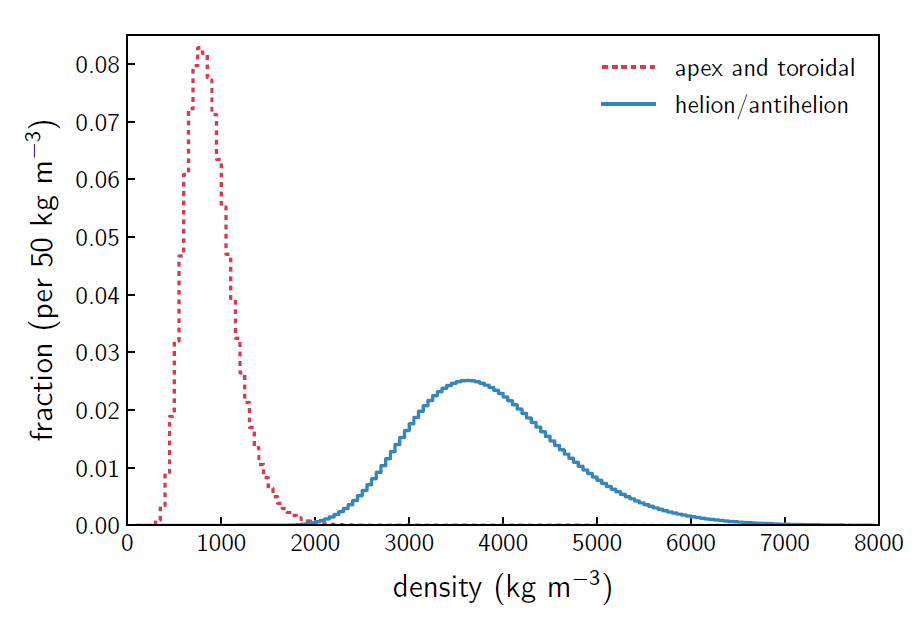
\includegraphics[scale=0.5]{MEM_UG_Fig2.5_density-distribution.PNG}
	\caption{Meteoroid density distribution according to the MEM3 User Guide. The apex and toroidal meteoroid sources constitute the low-density population, while the helion/antihelion source constitutes the high-density population. Each set of densities follows a log-normal distribution \citep[c.f. Figure 11,][]{moorhead2019nasa}.}\label{fig:MEM_UG_Fig2.5_density-distribution}
\end{figure}



\begin{figure}[!htb]
	\centering
	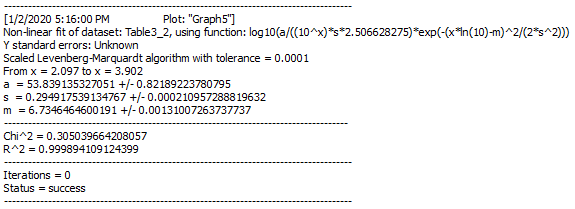
\includegraphics[scale=0.85]{Fit-to-MEM_low_dens.PNG}
	\caption{Non-linear fit of the low density profile in Figure \ref{fig:MEM_UG_Fig2.5_density-distribution} with Eq.\ \ref{eq:log-normal_distribution} in \textsf{SciDAVis}, giving the constants for $a\rightarrow A$, $s\rightarrow \sigma$, and $m\rightarrow \mu_\delta$.}\label{fig:Fit-to-MEM_low_dens}
\end{figure}

\begin{figure}[!htb]
	\centering
	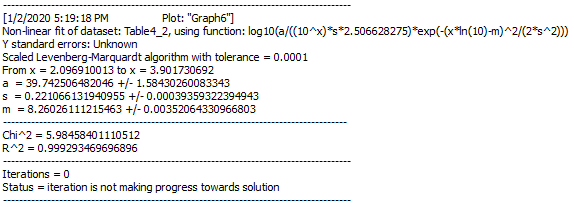
\includegraphics[scale=0.85]{Fit-to-MEM_high_dens.PNG}
	\caption{Non-linear fit of the high density profile in Figure \ref{fig:MEM_UG_Fig2.5_density-distribution} with Eq.\ \ref{eq:log-normal_distribution} in \textsf{SciDAVis}, giving the constants for $a\rightarrow A$, $s\rightarrow \sigma$, and $m\rightarrow \mu_\delta$.}\label{fig:Fit-to-MEM_high_dens}
\end{figure}
\clearpage

%%%%%%%%%%%%%%%%%%%%%%%%%%%%%%%%%%%%%%%%%%%%%%%%%%%%%%%%%%%%%%%%%%%%%%
\subsubsection{Mass Distribution}


From the MEM3 User Guide, the $g(m)$ flux of meteoroids larger than a limiting mass $m$ is obtained, originally from \cite{grun1985collisional}. The Gr{\"u}n interplanetary flux equation is given by
\begin{equation}\label{eq:Grun_flux}
g(m) = (c_4m^{\gamma_4}+c_5)^{\gamma_5} + c_6(m + c_7m^{\gamma_6} + c_8m^{\gamma_7})^{\gamma_8} + c_9(m + c_{10}m^{\gamma_9})^{\gamma_{10}},
\end{equation}
where the constants are $c_4 = 2.2\times 10^3$, $c_5 = 15$, $c_6 = 1.3 \times 10^{-9}$, $c_7=10^{11}$, $c_8=10^{27}$, $c_9 = 1.3\times 10^{-16}$, $c_{10} = 10^6$; and the exponents are $\gamma_4 = 0.306$, $\gamma_5 = -4.38$, $\gamma_6 = 2$, $\gamma_7 = 4$, $\gamma_8 = -0.36$, $\gamma_{9} = 2$, and $\gamma_{10} = -0.85$. Equation\ \ref{eq:Grun_flux} is applied to MEM's mass range and is shown in Figure \ref{fig:MEM_UG_Fig2.1_partile-mass-distribution}.

\begin{figure}[!htb]
	\centering
	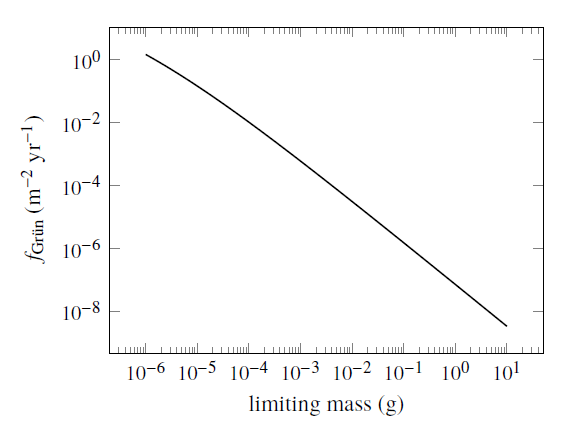
\includegraphics[scale=0.65]{MEM_UG_Fig2.1_partile-mass-distribution.PNG}
	\caption{The Gr{\"u}n interplanetary meteoroid flux as a function of limiting particle mass \citep[Figure 1]{moorhead2019nasa}, normalized to $1$ for a limiting mass equal to or greater than $1\mu$g.}\label{fig:MEM_UG_Fig2.1_partile-mass-distribution}
\end{figure}

	
%%%%%%%%%%%%%%%%%%%%%%%%%%%%%%%%%%%%%%%%%%%%%%%%%%%%%%%%%%%%%%%%%%%%%%
\subsection{Near-Earth Objects}\label{ssec:Near-Earth Objects}

The near-Earth objects (NEOs) described in this model consist of the small asteroids and comets between about $0.1$ m and $1000$ m diameter onto the lunar surface \citep{moorhead2020memo}. The speed and mass distributions (Sections \ref{sssec:NEO:Speed Distribution} and \ref{sssec:NEO:Mass Distribution}) were based on \cite{brown2002flux} and the Center for Near Earth Object Studies (CNEOS)\footnote{\url{https://cneos.jpl.nasa.gov/fireballs/}}, respectively. Both of the data sources are kinetic-energy-limited and correspond to the impact flux at the Earth's atmosphere, translated to fluxes onto the lunar surface \citep{moorhead2020memo}.

%%%%%%%%%%%%%%%%%%%%%%%%%%%%%%%%%%%%%%%%%%%%%%%%%%%%%%%%%%%%%%%%%%%%%%
\subsubsection{Speed Distribution}\label{sssec:NEO:Speed Distribution}

\begin{figure}[!htb]
	\centering
	\includegraphics[scale=0.45]{../NEA_Brown/vmass.png}
	\caption{Mass-limited speed distribution at the lunar surface.}\label{fig:vmass}
\end{figure}
The speed distribution of NEO's is shown in Figure \ref{fig:vmass}. The values (fraction of flux per bin) in each bin are midpoint values, where the bins have a size of 2 km s$^{-1}$. Note also that because the flux is a power law, this speed distribution is independent of limiting mass.



%%%%%%%%%%%%%%%%%%%%%%%%%%%%%%%%%%%%%%%%%%%%%%%%%%%%%%%%%%%%%%%%%%%%%%
\subsubsection{Mass Distribution}\label{sssec:NEO:Mass Distribution}


The mass-limited flux at the lunar surface can be shown to be \citep[see,][]{moorhead2020memo}
\begin{equation}\label{eq:NEO_mass_factor_int}
g_\leftmoon (m) = 2.89\times 10^{-11} \text{m}^{-2}\text{yr}^{-1}\cdot m^{-0.9},
\end{equation}
where $m$ is the mass of the impactor in kg. Since the mass-limited flux has a power-law index greater than $-1$, a maximum impactor size should be defined. An example of quantifying the largest size could be by computing the size that would have an $n-\%$ chance of hitting the Moon in $Y$ years. If $n = 5\%$ and $Y = 10$ years, then the largest size would be
\begin{align}
m_{max, kg} &= \left(\frac{2.89 \times 10^{-11} \text{m}^{-2}\text{yr}^{-1} \cdot 3.793\times 10^{13} \text{m}^{-2} \cdot 10 \text{yr}}{0.05}\right)^{1/0.9}\nonumber\\
&= 2.4\times 10^5 \text{ kg}.
\end{align}

If the NEO density is assumed to be $3.0$ g/cm$^2$ (which is the assumption used throughout the model), then this corresponds to a diameter of $5.3$ m.

\clearpage
%%%%%%%%%%%%%%%%%%%%%%%%%%%%%%%%%%%%%%%%%%%%%%%%%%%%%%%%%%%%%%%%%%%%%%
\subsection{Meteoroid Showers}\label{ssec:Meteoroid Showers}

The primary fluxes that originate from meteoroid showers can also produce ejecta. However, each different meteoroid shower has its own strength, duration, and time of year at which they occur. A prediction of the meteoroid shower fluxes as a function of time are compared to the sporadic meteoroids at different limiting energies, shown in Figure \ref{fig:2021_forecast_showers_southpole_moon} \citep{moorhead2020southpoleshower}.

\begin{figure}[!htb]
	\centering
	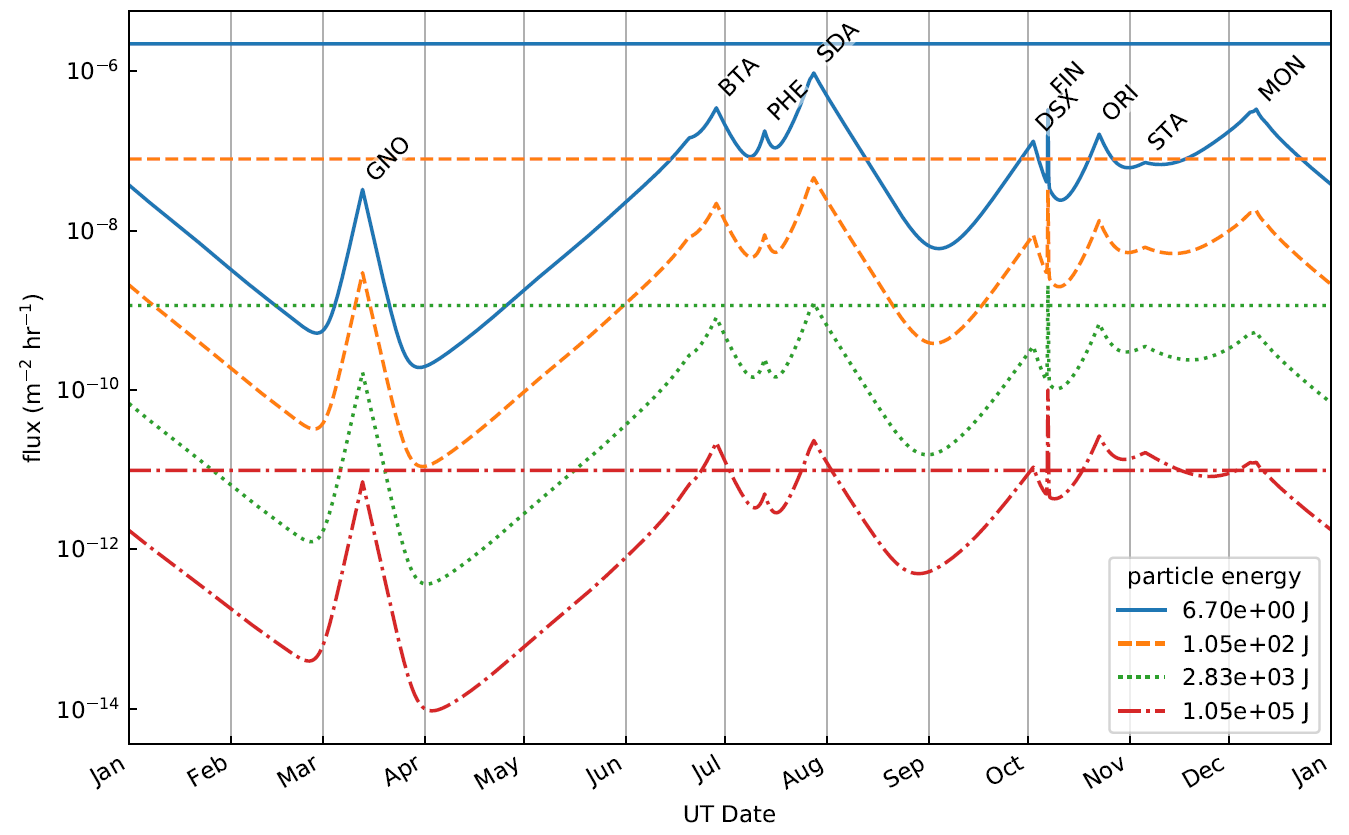
\includegraphics[width=1.0\linewidth]{../ShowerForecast/2021_forecast_showers_southpole_moon.PNG}
	\caption{Meteor shower flux (variable lines) and sporadic meteoroid flux (horizontal lines) over the course of 2021. Fluxes are quoted to four limiting particle kinetic energies; these kinetic energies correspond to particles with diameters of $0.04$ cm, $0.1$ cm, $0.3$ cm, and $1$ cm, assuming a density of $1$ g cm$^{-3}$ and a speed of $20$ km s$^{-1}$, \citep[see Figure 1,][]{moorhead2020southpoleshower}.}\label{fig:2021_forecast_showers_southpole_moon}
\end{figure}

At this time, it is assumed that the ejecta produced by meteoroid showers is small compared to the ejecta produced by the sporadic meteoroids. Further investigation may be warranted, however, short-term ejecta environments may need to include meteoroid showers during a particularly strong shower. These operational environments would be created on an as-need basis for lunar surface EVAs, similar to forecasts for meteoroid showers for ISS EVAs.

\clearpage
\end{document}